\documentclass[12pt, twoside]{article}
\input{../preamble}

\fancyhead[LE]{\thepage}
\fancyhead[RO]{Name: \hspace{4cm} \,\\ \hspace{2.9cm} \,}
\fancyhead[LO]{La Scuola d'Italia / Dr.\ Huson / IB Math: Probability \\* 11 March 2026}

\begin{document}
\subsubsection*{4.18 Homework: Probability Review}
\emph{This is practice for Friday's quiz. Show all working.}

\begin{enumerate}[itemsep=0.15cm]

%--- Problem 1: Venn diagram (mirrors Quiz P1) ---
\item In a class of 30 students, some study Spanish ($S$) and some study French ($F$).
Five students study both languages.

\begin{center}
\vspace{-0.2cm}
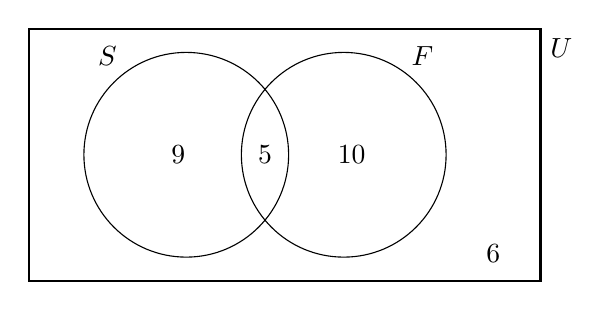
\begin{tikzpicture}
  \draw[thick] (0,0) rectangle (6.5,3.2);
  \node[anchor=north west] at (6.5,3.2) {$U$};
  \draw (2.0,1.6) circle (1.3cm);
  \node at (1.0,2.85) {$S$};
  \draw (4.0,1.6) circle (1.3cm);
  \node at (5.0,2.85) {$F$};
  \node at (1.9,1.6) {$9$};
  \node at (3.0,1.6) {$5$};
  \node at (4.1,1.6) {$10$};
  \node at (5.9,0.35) {$6$};
\end{tikzpicture}
\vspace{-0.2cm}
\end{center}

\begin{enumerate}[itemsep=0.1cm]
  \item Write down the number of students who study Spanish. \hfill [1]
  \item One student is chosen at random. Find the probability that
  \begin{enumerate}[label=(\roman*), itemsep=0.1cm]
    \item the student does not study Spanish; \hfill [1]
    \item the student studies Spanish or French, but not both. \hfill [2]
  \end{enumerate}
\end{enumerate}

\begin{tikzpicture}
  \draw (0,0) rectangle (15.5,3.5);
  \foreach \y in {1,2,3} \draw[dotted] (0.5,\y)--(15,\y);
\end{tikzpicture}

%--- Problem 2: Mutually exclusive (mirrors Quiz P2) ---
\item Events $C$ and $D$ are mutually exclusive with
$\mathrm{P}(C) = 0.35$ and $\mathrm{P}(D) = 0.25$.

\begin{enumerate}[itemsep=0.1cm]
  \item Write down $\mathrm{P}(C \cap D)$. \hfill [1]
  \item Find $\mathrm{P}(C \cup D)$. \hfill [2]
\end{enumerate}

\begin{tikzpicture}
  \draw (0,0) rectangle (15.5,2.5);
  \foreach \y in {1,2} \draw[dotted] (0.5,\y)--(15,\y);
\end{tikzpicture}

\newpage
%--- Problem 3: Venn with unknowns (mirrors Quiz P3) ---
\item In a group of 40 people, 22 like tea and 15 like coffee.
Eight people like both, as shown in the Venn diagram.
The values $\boldsymbol{a}$ and $\boldsymbol{b}$ represent numbers of people.

\begin{center}
\vspace{-0.2cm}
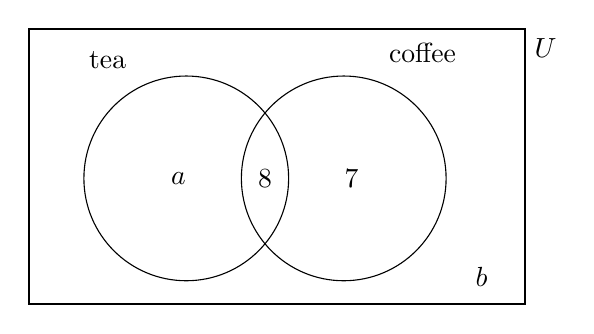
\begin{tikzpicture}
  \draw[thick] (0,0) rectangle (6.3,3.5);
  \node[anchor=north west] at (6.3,3.5) {$U$};
  \draw (2.0,1.6) circle (1.3cm);
  \node at (1,3.1) {tea};
  \draw (4.0,1.6) circle (1.3cm);
  \node at (5,3.2) {coffee};
  \node at (1.9,1.6) {$a$};
  \node at (3.0,1.6) {$8$};
  \node at (4.1,1.6) {$7$};
  \node at (5.75,0.35) {$b$};
\end{tikzpicture}
\vspace{-0.2cm}
\end{center}

\begin{enumerate}[itemsep=0.0cm]
  \item Find the value of $a$. \hfill [1]
  \item Find the value of $b$. \hfill [1]
  \item A person is chosen at random. Find the probability that the person
        likes coffee but not tea. \hfill [1]
  \item Find the probability that a person likes tea given that they like coffee. \hfill [2]
\end{enumerate}

\begin{tikzpicture}
  \draw (0,0) rectangle (15.5,3);
  \foreach \y in {1,2,3} \draw[dotted] (0.5,\y)--(15,\y);
\end{tikzpicture}

%--- Problem 4: Two-way table with independence test (mirrors Quiz P4) ---
\item The following table shows the travel method and punctuality of 20 students.

\renewcommand{\arraystretch}{1.6}
\begin{center}
\begin{tabular}{|r|c|c|c|}
    \hline
    & Punctual ($P$) & Sometimes late ($T$) & Total \\
    \hline
    Walk    & 3  & 7 & 10 \\
    \hline
    Bus     & 2  & 8  & 10  \\
    \hline
    Total   & 5  & 15 & 20 \\
    \hline
\end{tabular}
\end{center}

\begin{enumerate}[itemsep=0.0cm]
  \item Find the probability that a randomly chosen student walks to school
        and is punctual. \hfill [1]
  \item Find $\mathrm{P}(\text{punctual} \mid \text{bus})$. \hfill [2]
  \item Determine whether ``walks to school'' and ``is punctual'' are independent events.
        Show your working and justify your answer. \hfill [3]
\end{enumerate}

\begin{tikzpicture}
  \draw (0,0) rectangle (15.5,3);
  \foreach \y in {1,2,3} \draw[dotted] (0.5,\y)--(15,\y);
\end{tikzpicture}

%--- Problem 5: Tree diagram (mirrors Quiz P5) ---
\item A bakery makes bread using two ovens. Oven $A$ bakes $70\%$ of the loaves
and oven $B$ bakes the remaining $30\%$. The probability that a loaf from
oven $A$ is burnt is $0.04$. The probability that a loaf from oven $B$ is burnt
is $0.10$.

\begin{enumerate}[itemsep=0.3cm]
  \item Complete the tree diagram below, showing all probabilities. \hfill [3]

  \begin{center}
  \begin{tikzpicture}
    % Main branches
    \draw (0,0) -- (3.5, 2.0);
    \draw (0,0) -- (3.5,-2.0);
    % Oven A branches
    \draw (3.5, 2.0) -- (7.0, 3.2);
    \draw (3.5, 2.0) -- (7.0, 1.3);
    % Oven B branches
    \draw (3.5,-2.0) -- (7.0,-1.3);
    \draw (3.5,-2.0) -- (7.0,-3.2);
    % First-level labels
    \node[above] at (1.75, 1.0) {$0.7$};
    \node[below] at (1.75,-1.0) {$0.3$};
    \node[above left] at (3.5, 2.0) {\small Oven $A$};
    \node[below left] at (3.5,-2.0) {\small Oven $B$};
    % Second-level labels
    \node[above] at (5.25, 2.6) {$0.04$};
    \node[below] at (5.25, 0.8) {\rule{1.2cm}{0.4pt}};
    \node[above] at (5.25,-1.65) {\rule{1.2cm}{0.4pt}};
    \node[below] at (5.25,-3.5) {\rule{1.2cm}{0.4pt}};
    % Outcome labels
    \node[anchor=west] at (7.15, 3.2) {Burnt};
    \node[anchor=west] at (7.15, 1.3) {Not burnt};
    \node[anchor=west] at (7.15,-1.3) {Burnt};
    \node[anchor=west] at (7.15,-3.2) {Not burnt};
    % Composite probability blanks
    \node[anchor=west] at (10.0, 3.2) {$=$ \rule{1.8cm}{0.4pt}};
    \node[anchor=west] at (10.0, 1.3) {$=$ \rule{1.8cm}{0.4pt}};
    \node[anchor=west] at (10.0,-1.3) {$=$ \rule{1.8cm}{0.4pt}};
    \node[anchor=west] at (10.0,-3.2) {$=$ \rule{1.8cm}{0.4pt}};
  \end{tikzpicture}
  \end{center}

  \item A loaf is selected at random. Find the probability that the loaf is
  \begin{enumerate}[label=(\roman*), itemsep=0.1cm]
    \item burnt and from oven $A$; \hfill [2]
    \item burnt. \hfill [2]
  \end{enumerate}

  \item Given that a loaf is burnt, find the probability that it came from
        oven $A$. \hfill [3]
\end{enumerate}

\begin{tikzpicture}
  \draw (0,0) rectangle (15.5,4);
  \foreach \y in {1,2,3} \draw[dotted] (0.5,\y)--(15,\y);
\end{tikzpicture}

\newpage
%--- Problem 6: Without replacement (mirrors Quiz P6) ---
\item A bag contains 5 red marbles and 7 blue marbles. Two marbles are
drawn at random, one after the other, without replacement.

\begin{enumerate}[itemsep=0.1cm]
  \item Find the probability that both marbles are red. \hfill [2]
  \item Find the probability that both marbles are the same colour. \hfill [3]
  \item Find the probability that both marbles are red given that
        at least one marble is red. \hfill [3]
\end{enumerate}

\begin{tikzpicture}
  \draw (0,0) rectangle (15.5,11);
  \foreach \y in {1,2,...,10} \draw[dotted] (0.5,\y)--(15,\y);
\end{tikzpicture}

\end{enumerate}
\end{document}
